\chapter{phòng thí nghiệm kiểm định chất lượng sản phẩm}
\section{Tổng quan về phòng thí nghiệm kiểm định chất lượng}
phòng thí nghiệm kiểm định chất lượng là một trong những bộ phận chuyên môn tham gia trực tiếp vào công tác quản lý chất lượng sản phẩm tại Công ty TNHH Quốc tế Khánh Sinh. 
Với đặc thù hoạt động trong lĩnh vực sản xuất phân bón, công ty hiện sản xuất nhiều dòng sản phẩm với công thức và hàm lượng dinh dưỡng khác nhau. 
Vì vậy, việc kiểm tra và kiểm soát chất lượng nguyên liệu cũng như thành phẩm có vai trò quan trọng trong việc duy trì sự ổn định của sản phẩm trước khi đưa ra thị trường \cite{company-internal-document}.

phòng thí nghiệm phối hợp với Phòng Kỹ thuật và Bộ phận Sản xuất để thực hiện các hoạt động lấy mẫu, phân tích và đánh giá các chỉ tiêu chất lượng của nguyên liệu và sản phẩm. 
Kết quả kiểm nghiệm là một trong những cơ sở để xác định nguyên liệu có phù hợp để đưa vào sản xuất hay không, đồng thời đánh giá sản phẩm sau quá trình phối trộn có đáp ứng yêu cầu về thành phần và chất lượng đã đặt ra \cite{company-internal-document}.
Do danh mục sản phẩm của Khánh Sinh gồm nhiều nhóm phân bón nên các chỉ tiêu cần kiểm tra cũng thay đổi tùy theo từng sản phẩm.\cite{company-internal-document}.

Bên cạnh công tác kiểm tra thường xuyên, phòng thí nghiệm còn hỗ trợ công ty trong quá trình nghiên cứu, thử nghiệm và điều chỉnh công thức sản phẩm. 
Thông qua kết quả phân tích thực nghiệm, bộ phận kỹ thuật và sản xuất có thể đánh giá mức độ phù hợp của công thức phối trộn, từ đó thực hiện các điều chỉnh cần thiết trước khi sản xuất ở quy mô lớn. 
Có thể xem phòng thí nghiệm là một mắt xích quan trọng trong hệ thống kiểm soát chất lượng của công ty, kết nối giữa nguyên liệu đầu vào, quá trình sản xuất và chất lượng thành phẩm đầu ra \cite{company-internal-document}.

\section{Bố trí phòng thí nghiệm}

phòng thí nghiệm kiểm định chất lượng của Công ty TNHH Quốc Tế Khánh Sinh được bố trí nhằm phục vụ các hoạt động chuẩn bị mẫu, phân tích và kiểm soát chất lượng sản phẩm theo một quy trình làm việc thuận tiện và an toàn. 
Không gian phòng được phân chia thành các khu vực chức năng rõ ràng, bao gồm khu thiết bị phân tích, khu chuẩn bị mẫu, khu bảo quản mẫu, khu lưu trữ hóa chất và khu làm việc hành chính. 
Bàn chuẩn bị mẫu được đặt tại vị trí trung tâm, tích hợp các thiết bị thường xuyên sử dụng như máy xay xử lý nguyên liệu, máy khuấy từ kết hợp bếp gia nhiệt, máy đo pH và cân tiểu ly, giúp giảm quãng đường thao tác và tăng hiệu quả làm việc. 
Các thiết bị chuyên dụng như hệ thống chưng cất, tủ sấy, máy quang kế ngọn lửa và tủ hút được bố trí dọc theo khu vực riêng, trong khi tủ lạnh, tủ lưu mẫu và tủ hóa chất được tách biệt để thuận tiện cho bảo quản và hạn chế nguy cơ nhiễm chéo. 
Ngoài ra, phòng còn có một khu làm việc riêng dành cho máy tính và lưu trữ hồ sơ, giúp tách các hoạt động hành chính khỏi khu vực thao tác hóa chất và phân tích mẫu.

{\renewcommand{\figurename}{Sơ đồ}
\renewcommand{\thefigure}{\arabic{figure}}
\setcounter{figure}{1}
\begin{figure}[H]
  \centering
  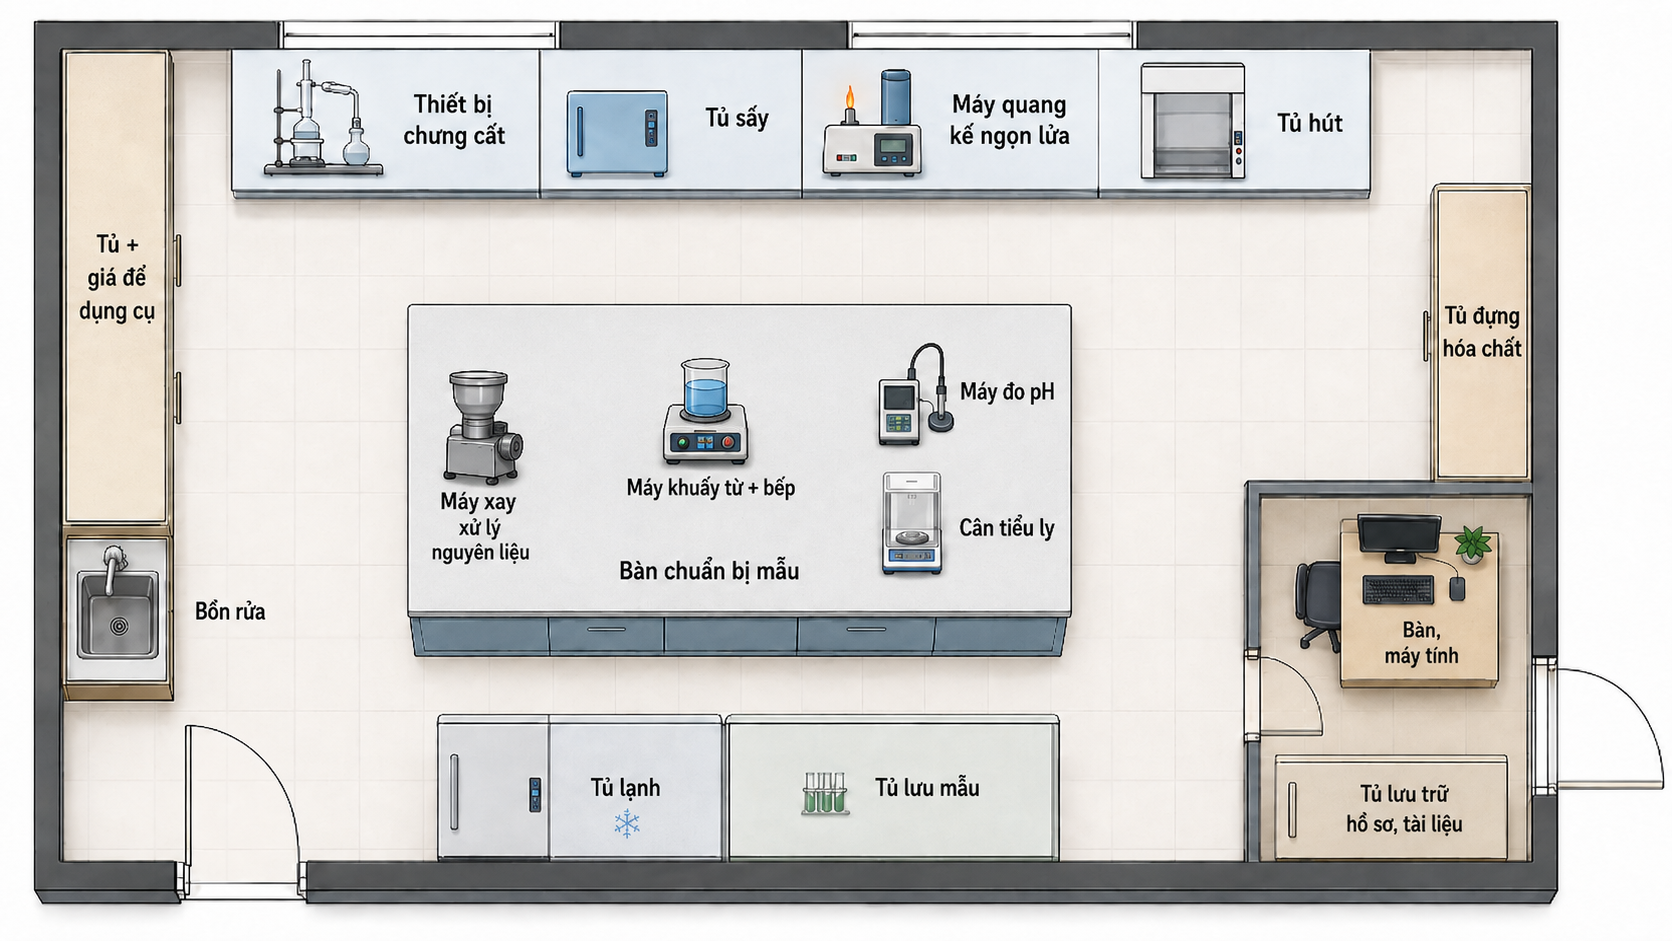
\includegraphics[width=\textwidth,height=0.72\textheight,keepaspectratio]{so do phong Lab.png}
  \caption{Bố trí phòng thí nghiệm kiểm định chất lượng sản phẩm.}
  \label{fig:lab-layout}
\end{figure}

}

\section{Nhiệm vụ và trách nhiệm của phòng thí nghiệm}
Nhiệm vụ của phòng thí nghiệm được thực hiện xuyên suốt các giai đoạn từ tiếp nhận nguyên liệu đến khi hoàn thiện thành phẩm. 
Các hoạt động chính có thể khái quát thành bốn nhóm \cite{company-internal-document}.

Thứ nhất, kiểm tra nguyên liệu đầu vào. 
phòng thí nghiệm tiến hành lấy mẫu và kiểm tra các chỉ tiêu cần thiết của nguyên liệu trước hoặc trong quá trình đưa nguyên liệu vào sản xuất. 
Kết quả kiểm nghiệm giúp đánh giá chất lượng nguyên liệu và cung cấp dữ liệu phục vụ tính toán, điều chỉnh công thức phối trộn khi cần thiết \cite{company-internal-document}.

Thứ hai, kiểm soát chất lượng trong quá trình sản xuất. 
Đối với các lô sản xuất, phòng thí nghiệm có thể tiến hành lấy mẫu tại các công đoạn phù hợp để đánh giá mức độ đồng đều và thành phần của sản phẩm. 
Nếu kết quả có sự sai lệch so với yêu cầu, thông tin được chuyển tới bộ phận kỹ thuật và sản xuất để xác định nguyên nhân và thực hiện biện pháp điều chỉnh \cite{company-internal-document}.

Thứ ba, kiểm tra thành phẩm. 
Sau khi hoàn thành quá trình sản xuất, mẫu đại diện của lô sản phẩm được phân tích nhằm xác định các chỉ tiêu chất lượng cần thiết. 
Kết quả kiểm nghiệm được sử dụng làm cơ sở đánh giá sự phù hợp của lô sản phẩm trước khi thực hiện các bước tiếp theo như đóng gói, lưu kho và đưa ra thị trường \cite{company-internal-document}.

Thứ tư, phòng thí nghiệm có nhiệm vụ quản lý và lưu trữ kết quả kiểm nghiệm. 
Các số liệu phân tích được ghi nhận theo từng mẫu hoặc từng lô sản xuất để phục vụ công tác theo dõi chất lượng, đối chiếu kết quả và truy xuất thông tin khi cần thiết. 
Việc duy trì hệ thống dữ liệu này cũng giúp công ty theo dõi sự ổn định của chất lượng sản phẩm qua các lô sản xuất khác nhau \cite{company-internal-document}.

\section{Nội quy an toàn trong phòng thí nghiệm}
Chỉ những người được phân công hoặc được phép mới được vào và làm việc trong phòng thí nghiệm.

Mặc đầy đủ trang bị bảo hộ cá nhân như áo blouse, găng tay, khẩu trang và kính bảo hộ khi thực hiện các thao tác có nguy cơ tiếp xúc với hóa chất.

Không ăn uống, hút thuốc hoặc để thực phẩm, đồ dùng cá nhân trong khu vực thí nghiệm.

Đọc kỹ nhãn, hướng dẫn sử dụng và thông tin an toàn của hóa chất trước khi tiến hành thí nghiệm.

Không tự ý sử dụng hóa chất, thiết bị hoặc thay đổi quy trình khi chưa được người phụ trách cho phép.

Hóa chất phải được dán nhãn đầy đủ, ghi rõ tên, nồng độ và các thông tin cần thiết; không sử dụng hóa chất không rõ nguồn gốc hoặc mất nhãn.

Các hóa chất dễ bay hơi, có mùi mạnh hoặc có nguy cơ gây hại phải được thao tác trong tủ hút.

Thiết bị như cân tiểu ly, máy đo pH, máy quang kế ngọn lửa, tủ sấy, máy khuấy từ và các thiết bị phân tích khác phải được sử dụng đúng hướng dẫn và kiểm tra tình trạng trước khi vận hành.

Không đặt hóa chất, mẫu hoặc dụng cụ không cần thiết lên bàn thiết bị để tránh nhiễm bẩn và ảnh hưởng đến kết quả phân tích.

Mẫu phân tích phải được mã hóa, ghi nhãn và quản lý rõ ràng để tránh nhầm lẫn giữa các mẫu.

Dụng cụ thủy tinh và dụng cụ phân tích phải được vệ sinh sạch sau khi sử dụng và đặt lại đúng vị trí quy định.

Khu vực bàn chuẩn bị mẫu phải được vệ sinh sau mỗi quá trình xử lý hoặc phân tích mẫu nhằm hạn chế nhiễm chéo.

Chất thải hóa học, dung dịch sau phân tích và chất thải thông thường phải được thu gom riêng theo đúng khu vực quy định; không tự ý đổ hóa chất xuống bồn rửa.

Không đổ hóa chất thừa trở lại chai chứa ban đầu để tránh làm nhiễm bẩn hóa chất gốc.

Sau khi sử dụng phải tắt nguồn điện, nguồn nhiệt và các thiết bị liên quan; kiểm tra lại tủ sấy, bếp gia nhiệt, máy khuấy từ và các thiết bị có khả năng sinh nhiệt.

Tủ hóa chất, tủ lưu mẫu và tủ lạnh phải được sắp xếp khoa học, có nhãn nhận diện và duy trì điều kiện bảo quản phù hợp.

Ghi chép đầy đủ kết quả kiểm nghiệm, thông tin mẫu, hóa chất sử dụng và các bất thường phát sinh trong quá trình phân tích.

Không tự ý mang mẫu, hóa chất, dụng cụ hoặc hồ sơ của phòng thí nghiệm ra khỏi khu vực khi chưa được phép.

Khi xảy ra sự cố như đổ hóa chất, vỡ dụng cụ, cháy, rò rỉ hoặc tiếp xúc hóa chất với cơ thể, phải dừng thao tác và báo ngay cho người phụ trách để xử lý.

Sau khi hoàn thành công việc, vệ sinh khu vực làm việc, sắp xếp dụng cụ đúng vị trí và rửa tay sạch trước khi rời phòng thí nghiệm.
